% A CW complex X with 1-skeleton X^1 (red) and four 2-cells (cyan).
% Source: book/tex/homology/cellular.tex (§ Digression: why are the groups equal?).
\documentclass[border=2mm]{standalone}
\usepackage{tikz}
\usepackage{amssymb}
\begin{document}
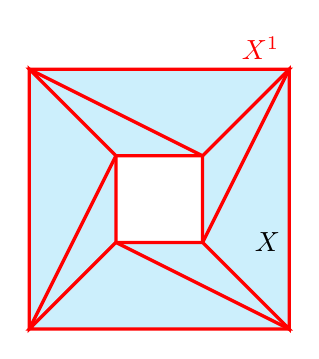
\begin{tikzpicture}[scale=0.55]
  \foreach \a in {0,90,180,270} {
    \begin{scope}[rotate=\a]
      \fill[cyan!20] (3,-3) -- (3,3) -- (1,1) -- (1,-1) -- cycle;
      \draw[red, line width=1.2pt] (3,-3) -- (3,3) -- (1,1) -- (1,-1) -- cycle;
      \draw[red, line width=1.2pt] (1,-1) -- (3,3);
    \end{scope}
  }
  \node at (2.5,-1) {$X$};
  \node[red, above left] at (3,3) {$X^1$};
\end{tikzpicture}
\end{document}
